 \begin{tabular}{SS[table-format=2]}
 \toprule
 	{Anno} & {Giorni Malattia} \\
 \midrule
 	1990 & 10,7 \\
 	1991 & 11,1 \\
 	1992 & 11,1 \\
 	1993 & 11,4 \\
 	1994 & 11,4 \\
 	1995 & 11,6 \\
	1996 & 11,5 \\ 
	1997 & 11,3 \\
	1998 & 11,2 \\
	1999 & 11,5 \\
	2000 & 11,6 \\
	2001 & 11,8 \\
	2002 & 12,1 \\
	2003 & 12,2 \\
	2004 & 11,8 \\
	2006 & 11,4 \\
	2007 & 11,4 \\
	2008 & 11,6 \\
	2009 & 11,7 \\
	2010 & 11,6 \\
	2011 & 11,6 \\
	2012 & 11,7 \\							  
	2013 & 11,8 \\
	2014 & 11,8 \\

 \bottomrule
 \end{tabular} 

 La regressione calcolata è di tipo logaritmica ed e' pari a:
 
 \[ f(x) = 0,293204 * ln(12,53 * 10^{15} * x )\]

 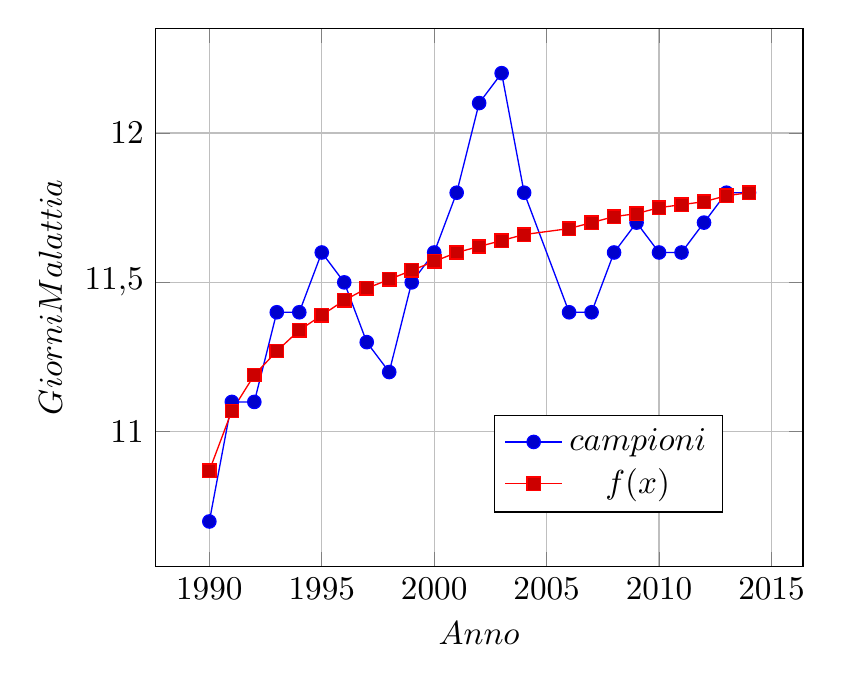
\begin{tikzpicture}[scale=1.2]
 \pgfkeys {
			/pgf/number format/.cd,
			set decimal separator={,{\!}},
			set thousands separator={}}
	\begin{axis}[ xlabel=$Anno$, ylabel=$Giorni Malattia$, grid=major, legend style={anchor=south, at={(0.7,0.1)}} ]
		
		\addplot coordinates{( 1990, 10.7) 
							  ( 1991, 11.1)
							  ( 1992, 11.1)
							  ( 1993, 11.4)
							  ( 1994, 11.4)
							  ( 1995, 11.6)
							  ( 1996, 11.5) 
							  ( 1997, 11.3)
							  ( 1998, 11.2)
							  ( 1999, 11.5)
							  ( 2000, 11.6)
							  ( 2001, 11.8)
							  ( 2002, 12.1)
							  ( 2003, 12.2)
							  ( 2004, 11.8)
							  ( 2006, 11.4)
							  ( 2007, 11.4)
							  ( 2008, 11.6)
							  ( 2009, 11.7)
							  ( 2010, 11.6)
							  ( 2011, 11.6)
							  ( 2012, 11.7)							  
							  ( 2013, 11.8)
							  ( 2014, 11.8)
							  };
							  
		\addplot coordinates{( 1990, 10.87) 
							  ( 1991, 11.07)
							  ( 1992, 11.19)
							  ( 1993, 11.27)
							  ( 1994, 11.34)
							  ( 1995, 11.39)
							  ( 1996, 11.44) 
							  ( 1997, 11.48)
							  ( 1998, 11.51)
							  ( 1999, 11.54)
							  ( 2000, 11.57)
							  ( 2001, 11.60)
							  ( 2002, 11.62)
							  ( 2003, 11.64)
							  ( 2004, 11.66)
							  ( 2006, 11.68)
							  ( 2007, 11.70)
							  ( 2008, 11.72)
							  ( 2009, 11.73)
							  ( 2010, 11.75)
							  ( 2011, 11.76)
							  ( 2012, 11.77)		
							  ( 2013, 11.79)
							  ( 2014, 11.80)
							  };
				\legend{$campioni$,$f(x)$}
	\end{axis}
\end{tikzpicture}

Quindi, si osserva che la nostra stima per l'anno 2016 di nostro interesse, il numero di giorni di malattia per singolo dipendente si assesta intorno ai:
 	
 \[		x = 26 \] 
 
( perche' il 2016 rappresenterebbe il 26 e-simo  valore nel nostro intervallo di campioni )
 \[		f(26) = 11,82 ( consideriamo 12 )	\]
 
consideriamo le seguenti ipotesi per ogni singolo centralinista: 
\begin{savenotes}
\begin{table}[htb]
\centering
 \caption{Assunzioni iniziali in un singolo mese}
 \begin{tabular}{p{7cm}D{,}{,}{5.2}}
 \toprule
 	& \multicolumn{1}{c}{\textbf{Quantita'}} \\
 \midrule 	
	\makebox[7cm][r]{Giorni lavorativi} & 18,50\\
	\makebox[7cm][r]{Giorni assenza} & 12,00\\	
 	\makebox[7cm][r]{Probabilita' di stipulare un contratto (\%)\footnote{dati istat}} & 15,60\\
 \bottomrule
 \end{tabular} 
\end{table}
\end{savenotes}
%
%	Numero chiamate centralinisti
%
\begin{savenotes}
\begin{table}[htb]
\centering
 \caption{Numero contratti centralinisti}
 \begin{tabular}{p{7cm}D{,}{,}{5.2}D{,}{,}{5.2}}
 \toprule
 	& \multicolumn{1}{c}{\textbf{Singolo Centralinisti}} & \multicolumn{1}{c}{\textbf{30 Centralinisti}} \\
 \midrule 		
	\makebox[7cm][r]{Numero chiamate giornaliere} & 94,00 & 2820\\
 	\makebox[7cm][r]{Numero chiamate mensili} & 1739,00\footnote{(94,00*18,50)} & 52170\\
 	\makebox[7cm][r]{Contratti stipulati mensilmente} & 271,29 & 8138,52\\ 	
 	\makebox[7cm][r]{Chiamate mensili in caso di assenza per 12 giorni} & 611,00\footnote{(94,00*(18,50-12,00))} & 18330\\
 	\makebox[7cm][r]{Contratti stipulati in caso di assenza per 12 giorni} & 95,32\footnote{(611*0,156)} & 2859,48\\ 	
 \bottomrule
 \end{tabular} 
\end{table}
\end{savenotes}

 
\begin{savenotes}
\begin{table}[htb]
\centering
 \caption{Variazione Fatturato}
 \begin{tabular}{p{8cm}D{,}{,}{5.2}D{,}{,}{5.2}}
 \toprule
 	& \multicolumn{1}{c}{\textbf{VAN PAREGGIO}} & \multicolumn{1}{c}{\textbf{VAN CASO REALE}} \\
 \midrule
 	\makebox[8cm][r]{Probabilita' di successo di un contratto (\%)} & 11,54 & 15,00\\
 \midrule
	\makebox[8cm][r]{Numero contratti stipulati (1 mese)} & 8138,52 & 8138,52\\
	\makebox[8cm][r]{Numero contratti stipulati (30 malati in 1 mese)} & 2859,48 & 2859,48\\
 \midrule	
	\makebox[8cm][r]{Numero contratti successo (1 mese)} & 939,50 & 1220,78\\
	\makebox[8cm][r]{Numero contratti successo (30 malati in 1 mese)} & 329,98 & 428,92\\
 \midrule	
	\makebox[8cm][r]{Fatturato Lordo (\euro) (1 mese)} & 75160,00 & 97662,40\\
	\makebox[8cm][r]{Fatturato Lordo (\euro) (30 malati in 1 mese)} & 26398,72 & 34313,76\\	
 \midrule	
	\makebox[8cm][r]{Fatturato Netto (\euro) (1 mese)} & 65314,04 & 84917,46\\
	\makebox[8cm][r]{Fatturato Netto (\euro) (30 malati in 1 mese)} & 22953,69 & 29835,81\\	
 \bottomrule
 \end{tabular} 
\end{table}\
\end{savenotes}